\documentclass[12pt,letterpaper]{article}
\usepackage[utf8]{inputenc}
\usepackage[margin=1in]{geometry}
\usepackage[margin=1cm]{caption}
\usepackage{amsmath}
\usepackage{amsfonts}
\usepackage{amssymb}
\usepackage{amsthm}
\usepackage{verbatim}
\usepackage{graphicx}
\usepackage{siunitx}
\usepackage{float}
% No paragraph tabs
\setlength{\parindent}{0pt}

% Define commands that will be widely used.
\newcommand{\br}{\ \\}
\newcommand{\tab}{\hspace*{2em}}
\newcommand{\bs}{\textbackslash}

\title{LaTeX is cool, I guess\dots}
\author{Rachel Domagalski}
\date{November 26, 2014}

\begin{document}
\maketitle

\begin{abstract}
    I ate French Toast for breakfast this morning.
\end{abstract}

\section{Lists}

Lists are useful, mkay?

\subsection{Bullets}

Things that I enjoyed about class this semester:
\begin{itemize}
    \item I enjoyed the purple couch.
    \item I enjoyed using vim.
\end{itemize}

\subsection{Numbered Lists}

Stuff I didn't like about the semester:
\begin{enumerate}
    \item Homework deadlines.
    \item emacs
\end{enumerate}

\section{Equations}

This is some hipster generalized version of the Euler-Lagrange equation:
\begin{equation}
    \sum_{j=0}^{n} \left(-1\right)^j \partial^j_{\mu_1\dots\mu_j}
    \left(\frac{\partial L}{\partial f_{i,\mu_1\dots\mu_j}}\right) = 0
\end{equation}

The variables $\mu_1\dots\mu_j$ are basically indices that span over the number
of variables in the equation.

\section{Tables}

This is a table:

\begin{table}[H]
    \centering
    \begin{tabular}{|c|c|c|}
        \hline
        Favorite Foods & Favorite Bands & Favorite IDL Commands \\
        \hline
        \textit{\textbf{Good}} sushi & Meshuggah & repstr() \\
        Waffle Fries & Nevermore & transpose() \\
        Pad Thai & Nightwish & print, \\
        Gordo's Quesadillas & Van Canto & return, \\
        \hline
    \end{tabular}
    \caption{Favorite genre: Metal. The fourth band is some a cappella
    metal-type stuff that's cheesy as fuck, but pretty good.}
\end{table}

LaTeX tables kind of suck. I'm done with LaTeX tables.

\section{Figures}

LaTeX figures have minds of their own.

\begin{figure}[H]
    \centering
    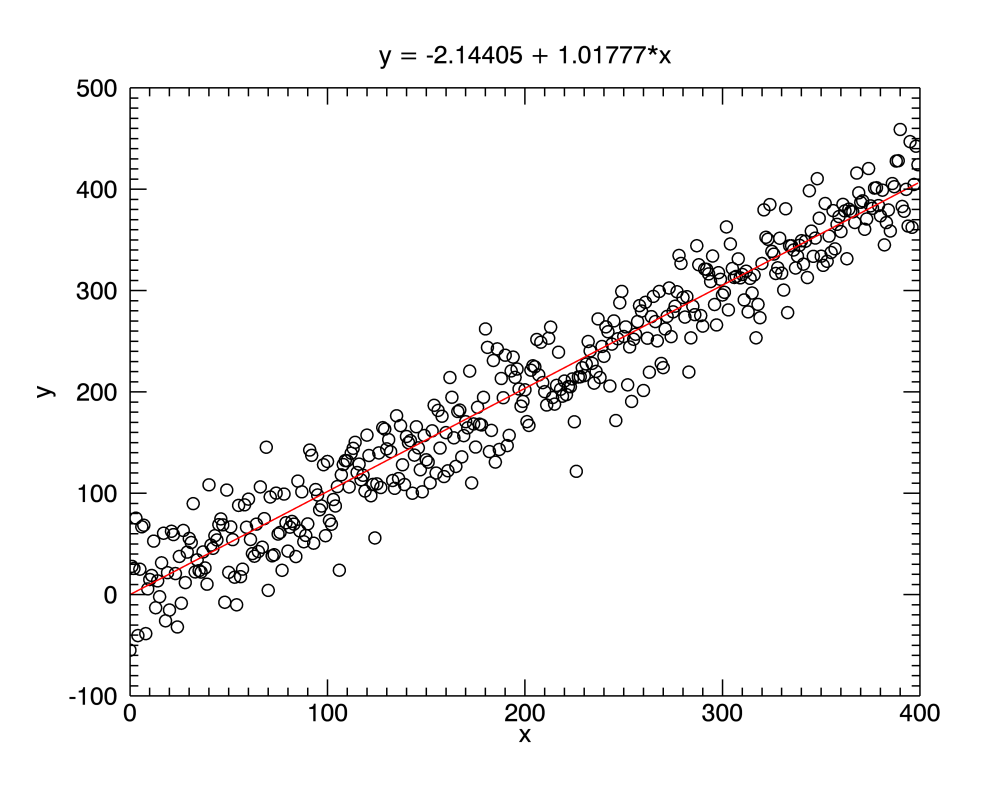
\includegraphics[width=0.6\textwidth]{lls-tut.png}
    \caption{This is a crappy PNG file from the linear least squares tutorial.}
\end{figure}

moar figures\dots

\begin{figure}[H]
    \centering
    \begin{minipage}[t]{0.475\textwidth}
        \centering
        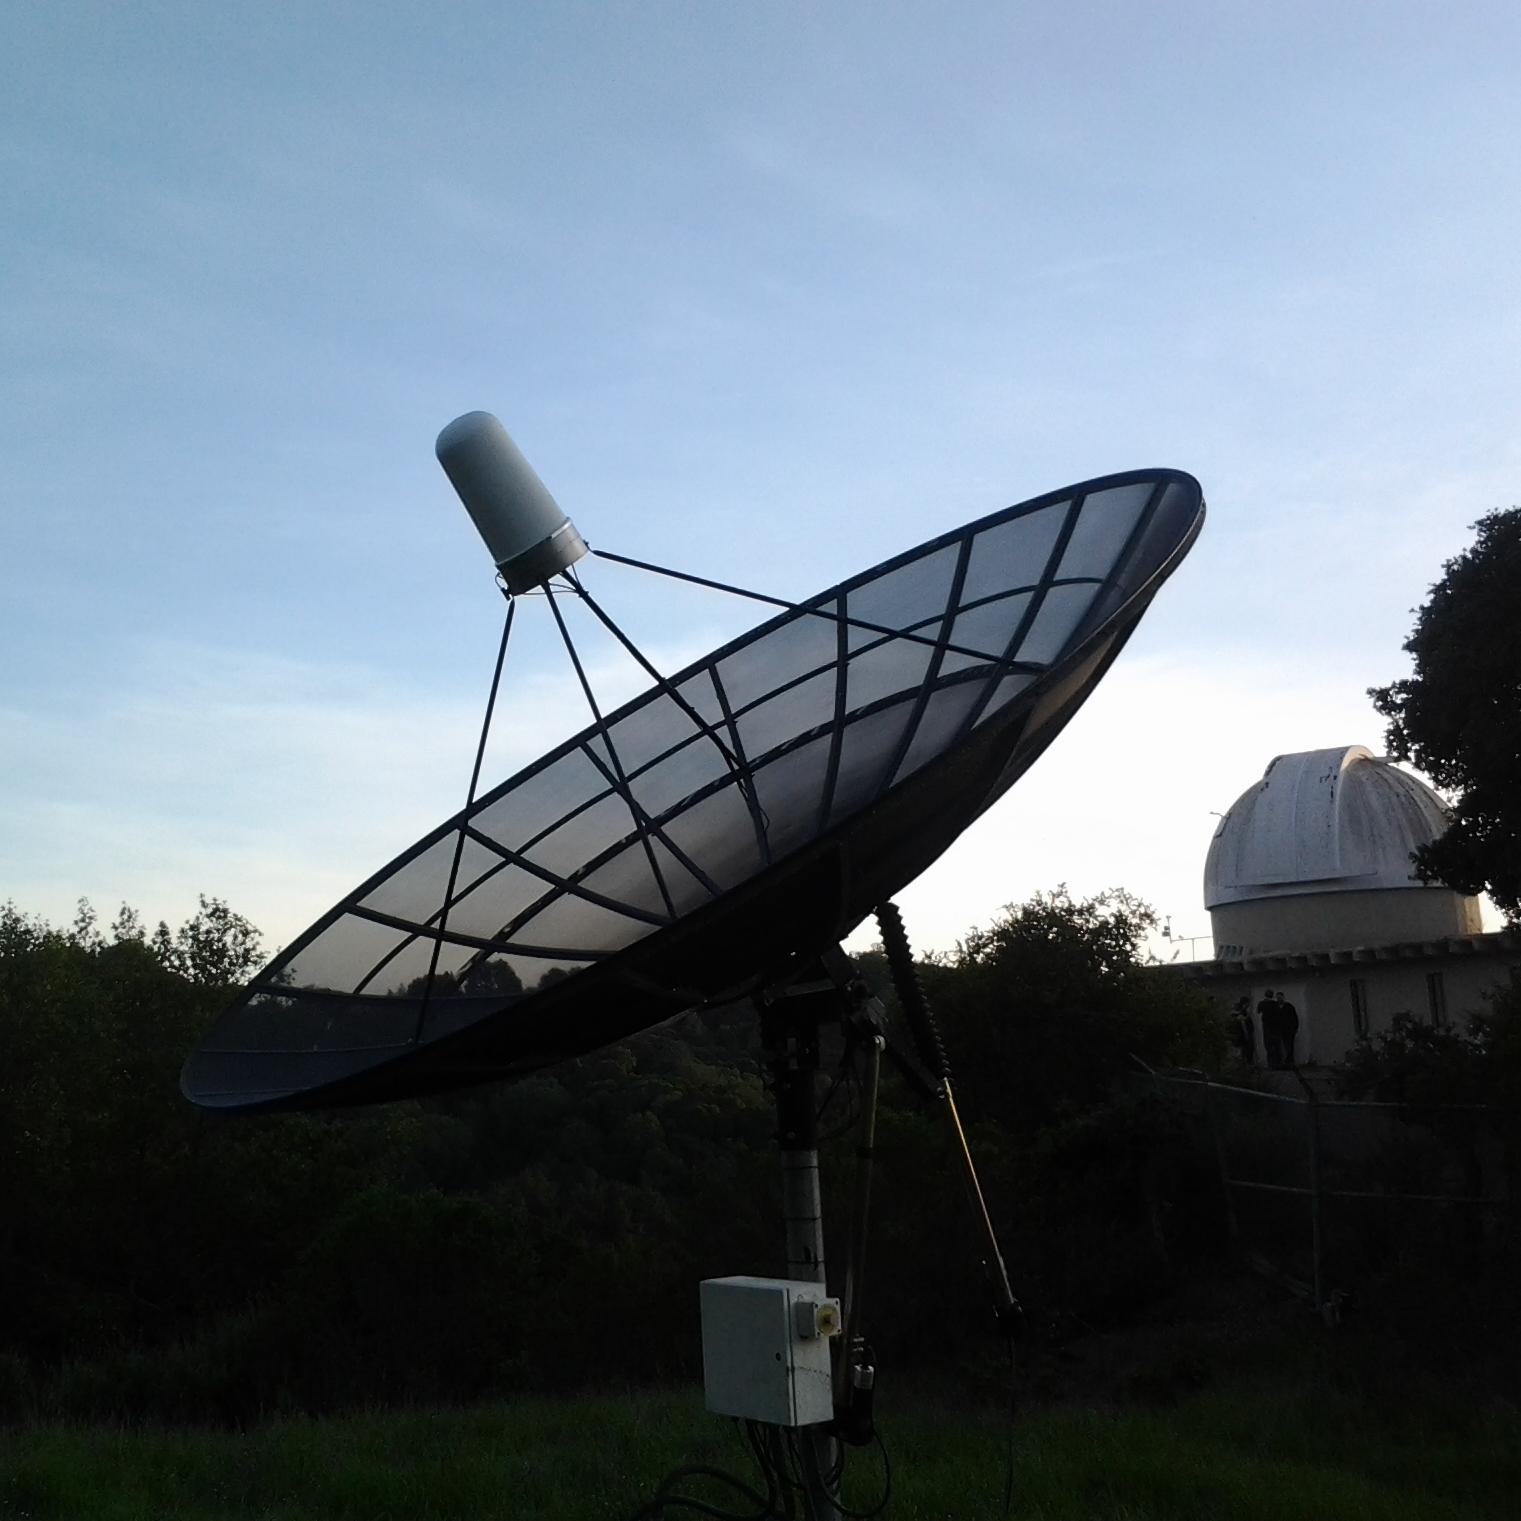
\includegraphics[width=\textwidth]{leuschner.jpg}
        \caption{This is a picture of the Leuschner radio telescope. The
        optical observatory can be seen in the background.}
    \end{minipage}
    \begin{minipage}[t]{0.475\textwidth}
        \centering
        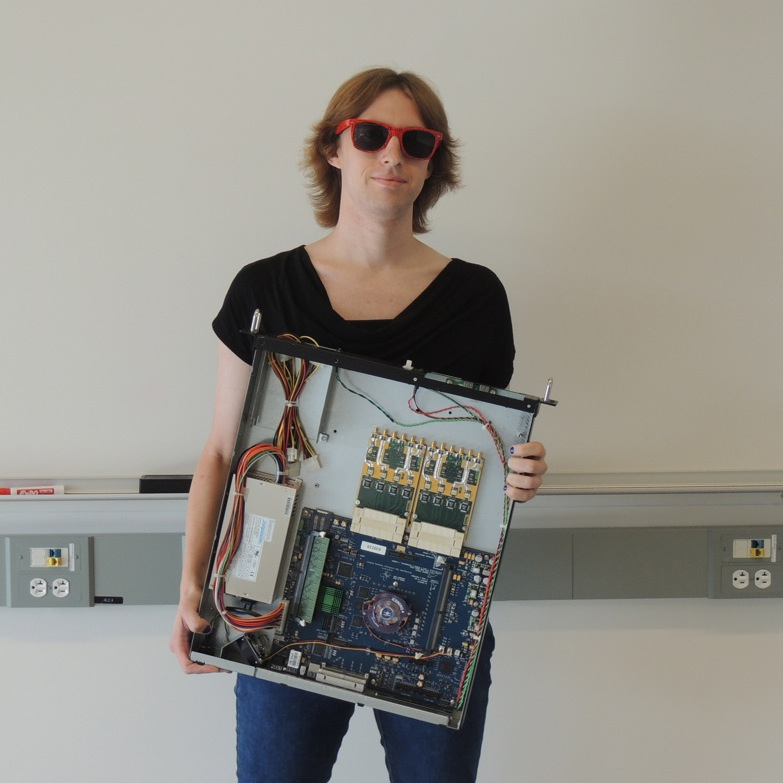
\includegraphics[width=\textwidth]{roach.jpg}
        \caption{This is a picture of me holding a ROACH board in my lab over in
        the new Campbell Hall.}
    \end{minipage}
\end{figure}

ok that's all folks\dots

\end{document}
